\documentclass{article}
\usepackage[utf8]{inputenc}
\usepackage{graphicx}
%\usepackage{xcolor}
\usepackage[a4paper,left=2cm,right=2cm,top=2cm,bottom=4cm]{geometry}



%%TODO 

% 50Ohm/HighZ




\begin{document}
\section*{Messtechnik LU Vorbereitung}
Datum: 9.1.2018

\subsection*{Wichtige Basics}
\begin{enumerate}
\item Trigger
\item bipolare Spannungsversorgung
\item Taskkopf abgleichen

\end{enumerate}
%\newpage
\subsection*{1. Labor }


\begin{itemize}
\item Messbereichserweiterung

%Innenwiderstand eines Voltmeters berechnet man wie folgt, man erwartet einen hohen Wert als Lösung: 
%\begin{equation}
%R_V = \frac{U_V}{U_{R1}} R_1
%\end{equation}
%Um den Einfluss des Voltmeters auf die Spannungsmessung zu ermitteln wird die Spannung am Voltmeter abgelesen und danach noch ein Voltmeter parallel geschaltet. Der Spannungsabfall am Voltmeter kann unter der Annahme das beide Widerstände gleich sind mit folgender Formel bestimmt werden: 

%\begin{equation}
%U_V = U  \frac{\frac{R_{i,v}}{2}}{R_M + \frac{R_{i,v}}{2}}
%\end{equation}

%\begin{figure}[h]
%\centering
%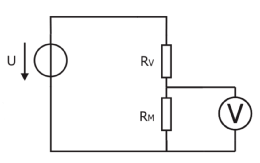
\includegraphics[width=5cm]{pic/messbereichserweiterung}
%\caption{ Schaltung Messbereichserweiterung }
%\begin{picture}(10,6)
%\put(35,85){\(R_1\)}
%\end{picture}
%\end{figure}
 Wird genutzt wenn die Spannung größer ist als der zu messende Messbereich. Es wird ein Vorwiderstand in Serie geschaltet, um einen Spannungsteiler zu erhalten. Um eine X-fache Spannungsmessbereichserweiterung durchzuführen muss der Vorwiderstand X-mal so groß sein wie der Messwiderstand. Eine X-fache Strommessbereichserweiterung kann man durchführen in dem man einen Vorwiderstand wählt der \(X^{-1}\)-mal so groß ist wie der Messwiderstand.  
 
\begin{figure}[h]
\centering
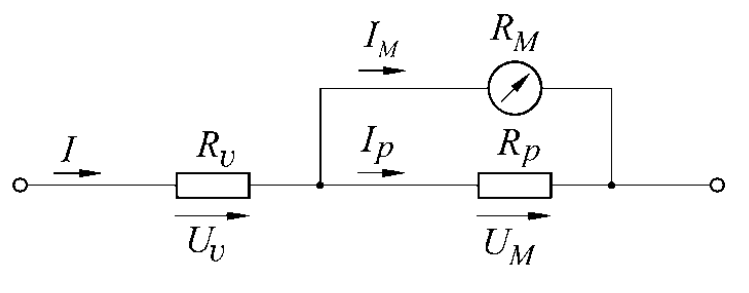
\includegraphics[width=8cm]{pic/messbereichserweiterung2}
\caption{Spannungsmessbereichserweiterung}
\end{figure}



% % % % % % % % % % % % % % % % % % % % % % % % % % % % % % % % %
\item Stromrichtig messen? 
\begin{figure}[h]
\centering
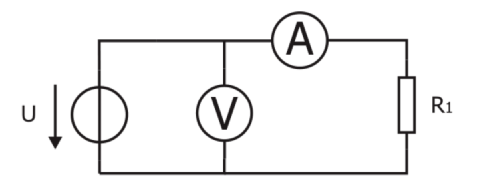
\includegraphics[width=5cm]{pic/irichtig}
\caption{ Schaltung zur Stromrichtigen Messsung }
\end{figure}

% % % % % % % % % % % % % % % % % % % % % % % % % % % % % % %
\item Spannungsrichig messen? 
\begin{figure}[h]
\centering
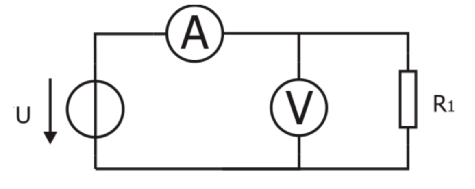
\includegraphics[width=5cm]{pic/urichtig}
\caption{ Schaltung zur Spannungsrichtigen Messsung }
\end{figure}

Der Widerstand vom Amperemeter ist idealerweise 0 \( \Omega \) und der Widerstandswert vom Voltmeter ist idealerweise \( \infty\ \).%\Omega \). 
% % % % % % % % % % % % % % % % % % % % % % % % % % % % % % % % % %
\item Messung von Vpp, Frequenz, Offset mittels Oszi (Sinus Signal)

Siehe Labor 6
% % % % % % % % % % % % % % % % % % % % % % % % % % % % % % % % % %
\item Frequenzgenerator - wann verwendet man 50Ohm / HighZ  und welche Auswirkung hat es?
?!?!?!?!?
Wir erwarten, dass der Effektivwert bei der "50\(\Omega\)" Einstellung in etwa doppelt so hoch sein wird, als bei der "HighZ" Einstellung, da wir damit dem Funktionsgenerator angeben, dass wir die Leitung mit 50Ω abgeschlossen haben, und dieser den 1:1 Spannungsteiler kompensieren versucht und die eingestellte Spannung verdoppelt.% Da unser Oszilloskop einen sehr hohen Eingangswiderstand hat, erwarten wir die doppelte Spannung messen zu können. Bei dem Sinus- und dem Dreiecksignal konnten wir das tatsächlich beobachten, jedoch scheint die Messung bei dem Rechtecksignal die Messung fehlerhaft erfolgt zu sein.
%Für hohe Frequenzen verwendet man idealerweise den 50 \(\Omega\) %Oszi
%%%%%%%%%%%%%%%%%%%%%%%%%%%%%%%%%
\item Bitauflösung Oszi: 

Die Formel lautet: 
\begin{equation}
Bitzahl = log_2 \left( \frac{V_{PP}}{U_{stufe}} \right)
\end{equation}

Um diese Formel verwenden zu können muss ein Signal gemessen werden. Davor muss der Tastkopf abgeglichen werden. Danach kann z.B. eine Ladekurve gemessen werden und das Signal soweit vergrößert werden das man die einzelnen Stufen sichtbar macht. 


\end{itemize}




% % % % % % % % % % % % % % % % % % % % % % % % % % % % % % % % % % % % % % % % % % % % % %

\subsection*{2. Labor }
\textbf{Bestimmen einer unbekannten Impendanz:} 

\textit{Signalform:} Am besten Sinusförmig!

\textit{Strommessung:} Um den Strom am Oszi darzustellen wird der Spannungsabfall eines Normwiderstandes (z.B.10\( \Omega \)) gemessen.  %Mithilfe eines Normwiderstandes (z.B. 10 \( \Omega \) ) 

\textit{Phasenwinkel:}  \(\Delta t \)…Differenz von Spannung zu Strom \& T…Periodendauer

\begin{equation} 
 \frac{\Delta t}{T} 360 = \Delta \varphi 
\end{equation}
\textbf{5/8 Methode:} Wenn man ein Signal so skaliert dass die Ladekurve von der linken unteren Ecke startet und den Endwert am obereren rechten Rand berührt kann man \( \tau \) direkt ablesen (\(\approx 63.2\% \)). 


\subsection*{3. Labor }

\begin{itemize}
\item Wie messen Sie CMRR? 

Common-Mode Rejection Ratio oder auch Gleichtaktunterdrückung kann bestimmt werden indem man die Differenzverstärkung und die Gleichtaktverstärkung misst. Danach setzt man in folgende Formel ein: 
\begin{equation}
CMRR = 20 \log \left( \frac{|Differenzenverstärkung|}{|Gleichtaktverstärkung|} \right) [dB]
\end{equation}
\textbf{Differenzenverstärkung:} An beiden Eingängen wird eine Spannung angelegt und der Ausgang gemessen, danach setzt man in folgende Formel ein: 
\begin{equation}
G_{diff} = \frac{U_a}{U_1-U_2}
\end{equation}

\textbf{Gleichtaktverstärkung:} An beiden Eingängen wird das selbe Signal angelegt und der Ausgang gemessen. Danach in die folgende Formel einsetzten: 
\begin{equation}
G_{gleich} = \frac{U_a}{U_e}
\end{equation}

% % % % % % % % % % % % % % % % % % % %

\item Offsetspannung, Gegentaktverstärkung und Gleichtaktunterdrückung messen

\textbf{Offsetspannung: } Die Eingänge kurzschließen und den Ausgang messen. 

\textbf{Gegentaktverstärkung \& Gleichtaktunterdrückung: } Siehe CMRR
% % % % % % % % % % % % % % % % % % % % % % % %
\item Abgleichbedingung 

Die Formel lautet: 
\begin{equation}
\frac{R_1}{R_2} = \frac{R_3}{R_4}  \quad \quad
U_D = U_2 - U_4
\end{equation}

% % % % % % % % % % % % % % % % % % % % % % % %
\item Gewichtsmessung mittels DMS 

\textbf{Halbbrücke:}  
\begin{figure}[h]
\centering
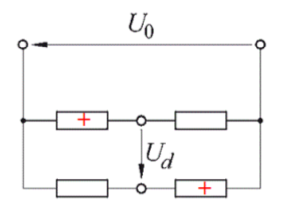
\includegraphics[width=5cm]{pic/halbbrucke.png}
\end{figure}

Schritt 1: Brücke kalibrieren, Messung(\textbf{\textit{M}}ittel\textbf{\textit{w}}ert) im Leerlauf und bei Belastung der Messbrücke. 

Schritt 2: Sensitivität berechnen, mit folgender Formel: 
\begin{equation}
E(\Delta m) = \frac{\Delta U_a}{\Delta m} \left[\frac{V}{g}\right]
\end{equation}
Sensitivität gilt nur für den angegebenen Bereich! 


Schritt 3: Offset messen. Eingänge auf Masse und Ausgang messen. Offsetspannung tritt auf weil es zu systematischen Fehlern im OPV kommt. 

Störeinflüsse einer 1/2 Brücke: 

Schritt 1: RMS Wert des Rauschens am Verstärkerausgang bei Umgebungstemperatur 

Schritt 2: Heizwiderstände anschließen. 

Schritt 3: Temperaturabhängigkeit von der Verstärkerausgangsspannung(Mittelwert)  wird mittels Variation der Temperatur ermittelt. 

Schritt 4: Gleichzeitig den RMS Wert des Rauschen messen. 

?Wie sieht die Rauschmessschaltung aus? 

\textbf{Vollbrücke:}
\begin{figure}[h]
\centering
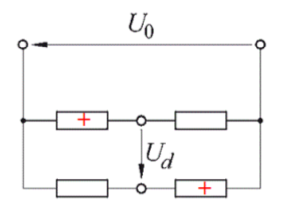
\includegraphics[width=5cm]{pic/halbbrucke}
\thicklines

\begin{picture}(10,6)
%\color{blue}
%\put(-108,14.2){\line(1,0){6}}
%\put(-49,47.2){\line(1,0){6}}
\put(-28,26){\line(1,0){6}}
\put(29,59.2){\line(1,0){6}}
\end{picture}
\end{figure}



Vollbrücke besteht aus 4 DMS und sonst alles gleich wie bei Halbbrücke. 








\end{itemize}


\subsection*{4. Labor }
\begin{itemize}
\item Was bedeutet DC-Modus am Oszi? 

DC-Modus am Oszi bedeutet dass das Oszi alle Signale ungefilter anzeigt. Wobei beim AC-Modus der Gleichanteil rausgefiltert wird und nur der Wechselanteil zeigt. 
%%%%%%%%%%%%%%%%%%%%%%%%%%%%%%%%%%%%%%%%%%
\item Wie wird bei AC der Gleich-Anteil entfernt und kann dies zu Problemen führen?

Durch einen, zum Signal, in Reihe geschalteten Kondensator wird der Gleich-Anteil entfernt. Dadurch wird ein eventueller Offset entfernt und dies könnte falsch interpretiert werden, allerdings wird die Messauflösung erhöht. 
%%%%%%%%%%%%%%%%%%%%%%%%%%%%%%%%%%%%%%%%%%
\item Was ist Differentielle Datenübertragung? 

Bei der Differentiellen Übertragung werden 2 Leitungen zur Datenübertragung verwendet. Auf Leitung 1 wird das Signal übertragen und auf Leitung 2 wird das invertierte Signal übertragen. 
%%%%%%%%%%%%%%%%%%%%%%%%%%%%%%%%%%%%%%%%%%
\item Was für Amplituden gibt es? 

\textbf{Spitzenwert}: ist der größte Maximalwert eines periodischen Signales innerhalb einer Periode. 

\textbf{Gleichrichtwert:} ist der Mittelwert des gleichgerichteten Signales. 

\textbf{Scheitelwert: } ist der maximale Augenblickswert eines Wechselsignals (Mittelwert=0). 

\textbf{Effektivwert: } ist der Scheitelwert mal \(\sqrt[]{2}\)

\textbf{Crestfaktor:} Spitzen- durch Effektivwert

\textbf{Formfaktor:} ist das Verhältnis von Effektiv- durch Gleichrichtwert. 
%%%%%%%%%%%%%%%%%%%%%%%%%%%%%%%%%%%%%%%%%%
\item Was ist Trigger

Der Trigger legt fest ab welcher Amplituden-Höhe das Signal erfasst wird. 
\textbf{Triggerarten}: Flanken, Level
\textbf{Trigger am Oszi:} Trigger Button \& Drehrad daneben. 


\end{itemize}





\subsection*{5. Labor }
% Vom Scheitelwert zu Effektivwert #Link https://www.elektrotechnik-fachwissen.de/wechselstrom/effektivwert-herleitung.php
\textbf{Signalgenerator:} \textit{Trig OUT} vom Oszi mit \textit{Trig} Eingang von DAQ, danach den \textit{Waveg Gen} Button \(\Rightarrow\) \textit{Settings, Trig Out} \(\Rightarrow\) \textit{WaveGen Sync \textbf{Aus}} 

\textbf{DAQ Karte} 

\textbf{Nyquist Frequenz} ist die Hälte der Abtastfrequenz und die Abtastfrequenz muss mind. doppelt so groß sein wie die größte vorkommende Frequenz. 


\subsection*{6. Labor }

\textbf{Messungen von Sinus Signal:}
\textit{Vpp:} FG \( \Rightarrow \) Oszi. Measurement Funktion Spitze Spitze auswählen, alternativ mit Curser messen.

\textit{Frequenz:} 1 Perioden Dauer am Bildschirm sichtbar machen, Div's zählen und ms in Hz umwandeln oder Measurement Funktion nutzen. 

\textit{Offset:} Signal einmal mit DC-Kopplung  und einmal mit AC-Kopplung einspeißen. Danach mit der Math-Funktion Subtraktion Kanal DC - AC wählen  und Measurement Scheitelwert auswählen. 

\textbf{Näherungssensor:} besteht aus seinem Sender (LED) und einem Empfänger (Fototransisor) die nebeneinander liegen. 

\textit{Funktionsweise:} Sender schickt Licht aus, welches vom Empfänger als reflektiertes Signal empfangen wird. Dabei ändert sich die Intensität je nach Einfallswinkel. 


\end{document}